\documentclass[conference]{IEEEtran}
\IEEEoverridecommandlockouts
% The preceding line is only needed to identify funding in the first footnote. If that is unneeded, please comment it out.
\usepackage{cite}
\usepackage{amsmath,amssymb,amsfonts}
\usepackage{algorithmic}
\usepackage{graphicx}
\usepackage{textcomp}
\usepackage{xcolor}
\def\BibTeX{{\rm B\kern-.05em{\sc i\kern-.025em b}\kern-.08em
		T\kern-.1667em\lower.7ex\hbox{E}\kern-.125emX}}
	
%\usepackage[margin=0.9in]{geometry}
%\usepackage{hyperref}
%\usepackage{natbib}
%\usepackage{xcolor}
\definecolor{citeblue}{RGB}{17,127,197}
\usepackage{hyperref}
\hypersetup{
	colorlinks,
	citecolor=citeblue,
	filecolor=black,
	linkcolor=black,
	urlcolor=blue
}

\usepackage{listings}
\lstset{
	basicstyle=\ttfamily,
	columns=fullflexible,
	language=python,
	numbers=none,
	stepnumber=1,
	frame=none,
	breaklines=true,
	showstringspaces=false,
	postbreak=\mbox{\textcolor{red}{$\hookrightarrow$}\space},
	basicstyle=\footnotesize\ttfamily,
	keywordstyle=\bfseries\color{green},
	commentstyle=\itshape\color{red},
	identifierstyle=\color{blue},
	stringstyle=\color{black},
}



\begin{document}
	
	\title{Image Super-resolution using \\ Generative Adversarial Networks\\
		{\large PG-Independent Study Report}
		\vspace{-3mm}
		%\thanks{PG-Independent Study}
	}

	
	\author{\IEEEauthorblockN{Ankit Pant}
		\IEEEauthorblockA{2018201035}
			\textit{M.Tech. Computer Science \& Engineering}\\
			International Institute of Information Technology, Hyderabad \\
			%ankit.pant@students.iiit.ac.in \\
				Supervised by: Dr. Pawan Kumar
		}
		
	
	\maketitle
	
	\begin{abstract}
		Artificial Intelligence (AI) and Machine Learning (ML) have taken the world by storm. AI and ML are being applied to new applications at a very fast rate. One such application is Image Super-resolution. This application involves enhancing the details in an image and converting a low-resolution image to a higher resolution image. Generative Adversarial Networks (GANs) are novel models that show a lot of promise in such applications. The PG-Independent Study undertaken attempts to explore GANs and apply them to the field of image super-resolution. Images of people (portraits, selfies, etc.) are used as datasets and the study attempts to enhance such images.
	\end{abstract}
	
	\begin{IEEEkeywords}
		Image Super-resolution, Generative Adversarial Networks, image-enhancement, portraits, GANs
	\end{IEEEkeywords}
	
	\section{Introduction}
		Artificial Intelligence (AI) and Machine Learning (ML) has come a long way since their inception. Various models, finding various applications have been developed and have also increased tremendously in their complexity. The greatest advantage of this rapid development has been the application of AI and ML in various fields, from Computer Vision to Speech Processing, from Expert Systems to Natural Language Processing.
		\par Among the various models developed, Generative Adversarial Models (GANs) are of significant interest. GANs work on the premise of having two models that are competing with each other in a form of a game. GANs have come a long way since they were proposed in 2014 by Goodfellow et al. \cite{b1}. One of the major problems with GANs had been the slower learning rate. This can be circumvented by pre-training the generator and the discriminator.
		\par GANs have been used in a variety of applications. They fare well in tasks that require creation and enhancements. One such application is \emph{image super-resolution} which involves enhancing low resolution images and converting them to higher resolution images containing more detail. With the amount of data being generated, it is critical for various services to compress the data. Such compression leads to loss of detail and once at source, this ill effect of compression can be neutralised by using image super-resolution at source.
		\par This PG-Independent Study aims to cover Generative Adversarial Networks and Image Super-resolution (in moderate detail) and create a ML model that can enhance portrait images (including selfies) of (majorly) human subjects. A web application has also been created (using Python) that allows the user to input a low quality image and enhance it. Further details can be found in the subsequent sections.
	
	\section{Literature Review}
	
		\subsection{Generative Adversarial Networks (GANs)}
			Generator Adversarial Networks (GANs) are ML models that are composed of a \emph{generator} and a \emph{discriminator} working in tandem to learn the features of the task given to it and has a variety of applications \cite{b2}. The \emph{generator} model that attempts to recreate the ground truth (often from random noise) and the \emph{discriminator} (or critic) that attempts to distinguish between the ground truth and the output of the generator. Both the generator and the discriminator may be pre-trained to improve performance. GANs work by repeatedly running a training loop which can be loosely described as follows:
			\begin{enumerate}
				\item The generator attempts to create the ground truth.
				\item The discriminator takes this generated image and compares it to the ground truth
				\item Repeat 1. based on the feedback from 2.
			\end{enumerate}
			Ideally the training loop needs to be stopped when the discriminator outputs $0.5$ i.e. it can no longer differentiate between the ground truth and the generated image.
			\par Multiple variations of GANs have been developed including Deep convolutional GANs (DCGANs) \cite{b3}, Wasserstein GAN (WGANs) \cite{b4}, and Softmax GAN \cite{b5}.
			
		\subsection{Image Super-resolution}
			Image super-resolution \cite{b6} can be simply defined as conversion of one or more low resolution images to a high resolution image. The resultant images are larger and have more detail. This technique can be used to enhance videos as well.
			
			\subsubsection{Techniques}
				The various techniques for image super-resolution includes:
				\begin{itemize}
					\item \textit{Single Frame Super Resolution:} This method involves smoothing, interpolation and sharpening to estimate the details that are not present.
					\item \textit{Multi Frame Super Resolution:} This method involves using multiple low-resolution images of the same scene albeit each of those images taken from different angles (shifted with sub-pixel precision). These images are then combined to get an enhanced image.
				\end{itemize}
			
			\subsubsection{Applications}\label{srapplications} The various applications of image super-resolution includes:
			\begin{itemize}
				\item Enhancing photographs and self-portraits of people
				\item Enhancing surveillance footage
				\item Enhancing medical diagnostic images
				\item Enhancing astronomical and remotes sensing images
				\item Enhancing low resolution videos
			\end{itemize}
		
	\section{Methodology}
		Image enhancement is attempted during the course of the study using a Generative Adversarial Network. The approach consists of these steps:
		\begin{itemize}
			\item Creating and training the ML model
			\item Creating the Web application to use the model
		\end{itemize}
	 	\par The ML model has been created in Python using fast.ai libraries (that in-turn uses Pytorch) \cite{b7}. The code is in the form of Jupyter Notebook and that allows for easy reproduction. Google Colab was used as the platform to train and test the model. The ML model currently can scale low-resolution images to a resolution of $512 * 512$ pixels. This limitation is due to the computing resources that were available during the training of the model. The model can be easily extended to upscaling to higher resolutions in the presence of more powerful hardware.
	 	\par The Web Application has been created in Python and is run by deploying it in a Docker container (environment). Docker ensures that all the necessary libraries and dependencies are installed in the first run of the application.
	 	\par The following sub-sections provide further details.
	 	
		\subsection{Overview of the algorithm}
			The algorithm to create the ML model consists of the following steps:
				\begin{enumerate}
					\item The high resolution images ($1024 * 1024$ pixels)\cite{b8} are first taken and converted to low resolution images ($128 * 128$) pixels. The high resolution images act as the ground truth and the low resolution images act as training data.
					\item The generator model is then individually trained on this training dataset. The resultant generated images are then saved.
					\item The discriminator model is then individually trained on the generated images and original images so that it can learn to determine the generated images from original images.
					\item Both the generator and discriminator are then combined as a GAN and trained.
					\item The generated images obtained from the GAN are then saved for comparison with original noisy images. The trained model was saved as well.
					\item Another step to upsample the images was applied that converts the images to the resolution of ($512 * 512$ pixels). This model was also saved.
					\item A test dataset \cite{b9} consists of low resolution images ($306 * 306$) pixels and was used to visually see the output of the model.
					\item The saved models were then imported to the web application as used to enhance the images provided by the user.
				\end{enumerate}
		\subsection{Architecture of the ML model}
			The ML model consists of three sub-models. The generator, the discriminator, and the up-sampler. All the three models are based on the models created in the fast.ai library\cite{b7}.
			
			\par The \emph{generator} model is based on the UNet model\cite{b10}. It uses Resnet34\cite{b11} as the base architecture and Mean Squared Error (MSE)\cite{b12} as the loss function. This model is pre-trained for 7 cycles with varied learning rated (from $10^{-5}$ to $10^{-3}$).
			
			\par The \emph{discriminator} model uses the basic \emph{gan\_critic} provided by the fast.ai library\cite{b7}. It uses Cross Entropy\cite{b13} as the loss function and is pre-trained for 8 cycles with varied learning rated (from $10^{-6}$ to $10^{-3}$).
			
			\par The \emph{up-sampler} model is based on the UNet model\cite{b10}. It uses VGG-16\cite{b14} as the base architecture and Mean Squared Error (MSE)\cite{b12} as the loss function. This model is pre-trained for 11 cycles with varied learning rated (from $10^{-6}$ to $10^{-3}$).
			
			\par There were certain issues with saving the aforementioned \emph{up-sampler} model to be used with the web-application. Hence another up-sampler model was created to be used specifically for the web-application. This model was created using the upsampling model available in the fast.ai library\cite{b7} with modifications. However, this model does not perform as well as the aforementioned up-sampler model based on UNet.
			
			\par The architecture can be summarized in the figure \ref{arch-fig}.
			
				\begin{figure}[htbp]
				\centerline{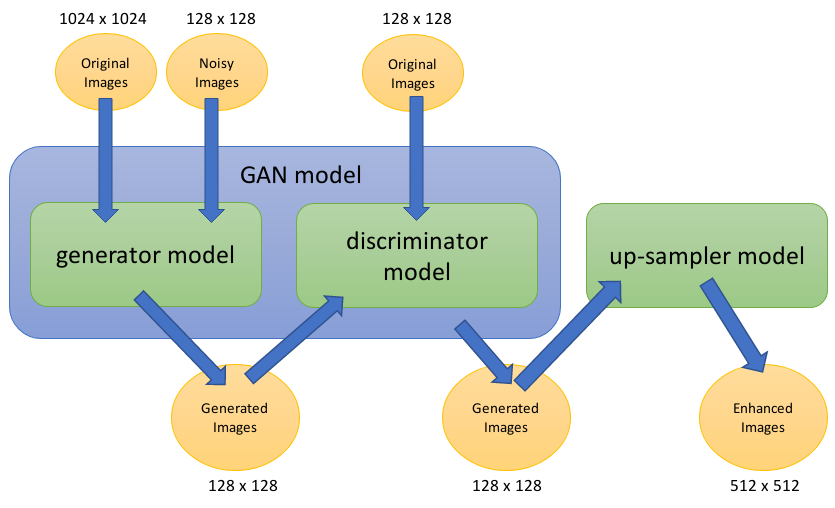
\includegraphics[width=25em]{arch_srgan.png}}
				\caption{Architecture of ML model}
				\label{arch-fig}
			\end{figure}
			
		\subsection{Training and Test Datasets}
			Different open source datasets were used for training and testing purposes.The details of the datasets is as follows:
			
			\subsubsection{Training Dataset}
				The training dataset comprised of 1600 images from the Flickr-Faces-HQ Dataset. It contains high quality images and was created originally as a benchmark for GANs\cite{b8}.
				
			\subsubsection{Test Dataset}
				The test dataset comprised of 300 images from the Selfie Data Set\cite{b9}. It contains low quality images.
				
		\subsection{Measures to compare images}
			Different measures were used to compare the enhanced images to the original images as well as the low-resolution images to the original images. The measures used were:
			
			\subsubsection{MS-SSIM}
				Multi Scale Structural Similarity (MS-SSIM) index is used to predict the perceived quality of images and videos \cite{b15}. The values of MS-SSIM range from $(-1$ to $1)$ with 1 only possible in-case of identical images. Higher values indicate better similarity and hence less error.
				
			\subsubsection{MSE}
				Mean Squared Error(MSE) is used to mathematically differentiate two images by comparing the value in each pixel \cite{b12}. The closer the values are to 0, the more identical the compared images are, with 0 being identical images.
				
			\subsubsection{PSNR} 
				Peak Signal to Noise Ratio (PSNR) can also be used to compare two images. In general it is described as the ratio between the maximum possible power of a signal and the power of corrupting noise\cite{b16}. Higher values of PSNR indicate higher fidelity and hence less error.
				
			\subsubsection{L1}
				L1 also know as Least Absolute Deviations (LAD) or Least Absolute Errors (LAE) \cite{b17, b18}, is a regularization technique that can be used to compare images. The closer the values are to 0, the more identical the compared images are, with 0 being identical images. 
				
			
			
		\subsection{Creating the Web Application}
			The web application was created using Python and was deployed using Docker. The web application allows the user to pick a low-resolution image and enhances it to an image of resolution ($512 * 512$ pixels). The images \ref{appui1-fig} and \ref{appui2-fig} shows the user interface for the web application.
			\begin{figure}[htbp]
				\centerline{
\includegraphics[width=25em]{webapp_ui1.png}}
				\caption{Web application UI (no image chosen)}
				\label{appui1-fig}
			\end{figure}
			\begin{figure}[htbp]
				\centerline{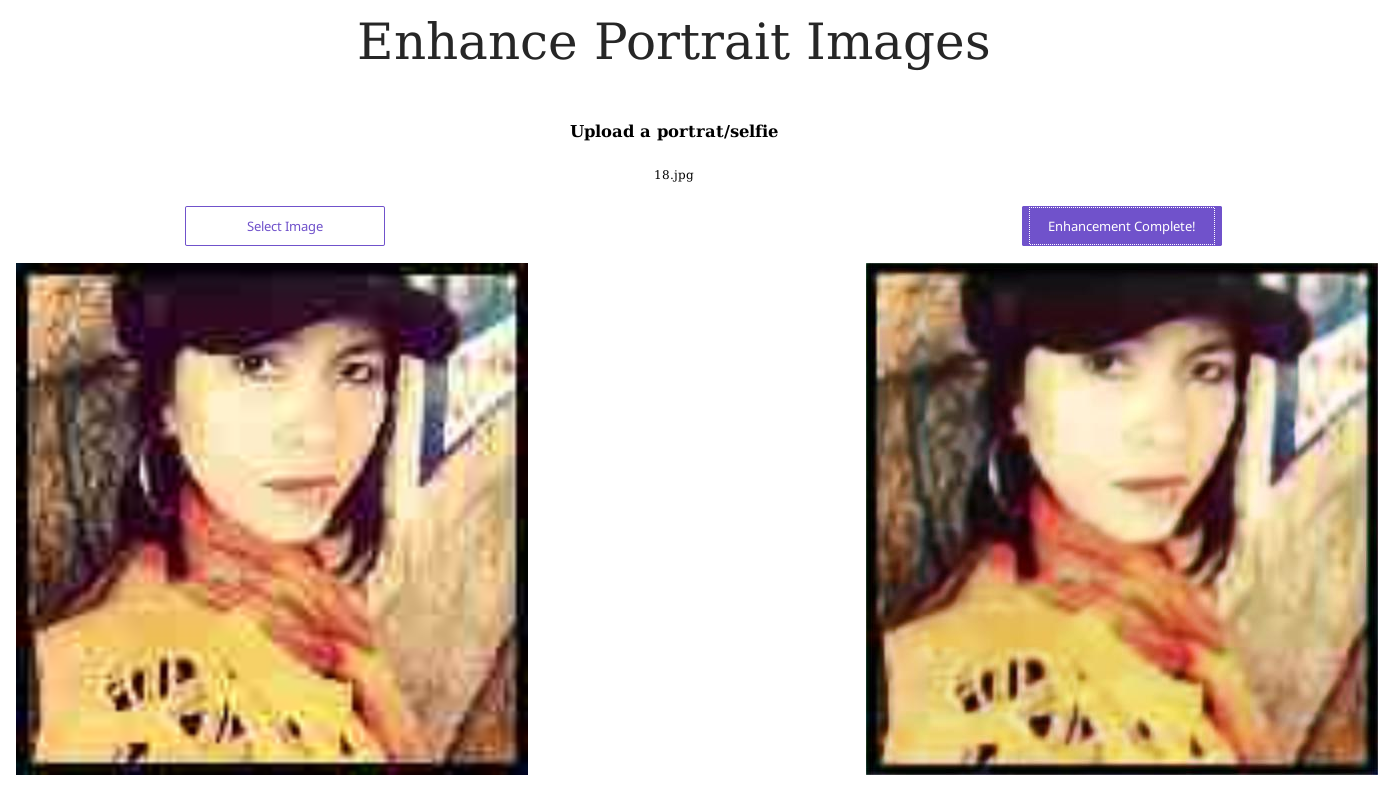
\includegraphics[width=25em]{webapp_ui2.png}}
				\caption{Web application UI (after enhancing image)}
				\label{appui2-fig}
			\end{figure}
		
		
	\section{Experimentation}
		The ML model was trained in Google Colab. The specification of the hardware is as follows:
		\begin{itemize}
			\item RAM: 25.51 GB
			\item VRAM (GPU Memory): 12 GB
			\item Disk Space: 358.27 GB
		\end{itemize}
		
		The approximate training times of various models are given below:
		\begin{itemize}
			\item Generator model (individual): 13 minutes
			\item Discriminator model (individual): 18 minutes
			\item GAN: 48 minutes
			\item Up-sampler: 135 minutes
		\end{itemize}
	
		After the ML models were trained, they were saved so that they could be used to make prediction on test dataset or other unseen data.
		
	\section{Results}
		Two results were obtained during the study. One was the comparison between the low resolution images and the images obtained by the pre-trained generator (before applying GAN model), with the original images, the results of which are given in table \ref{tab1}. The second was a comparison between the low resolution images (directly resized) and the enhanced images, with the original images, the results of which are given in table \ref{tab2}.
		
		\begin{table}[htbp]
			\caption{Comparison between low-res and initially generated images}
			\begin{center}
					\begin{tabular}{| p{0.2cm}| p{2cm}| p{1.2cm}|p{1.5cm}|p{1.2cm}|p{1.5cm}|}

						\hline

						 & Image type      & average SSIM & average MSE  & average PSNR & average L1 \\ \hline

						1      & Low-res Image     & 0.127138     & 25652.102085 & 4.295813     & 3.603803e+06     \\ \hline

						2      & Generated Image & 0.135904     & 25757.227375 & 4.304846     & 3.611744e+06     \\ \hline
 

					\end{tabular}
				\label{tab1}
			\end{center}
		\end{table}
		
		\begin{table}[htbp]
			\caption{Comparison between low-res and enhanced images}
			\begin{center}
				\begin{tabular}{| p{0.2cm}| p{2cm}| p{1.2cm}|p{1.5cm}|p{1.2cm}|p{1.5cm}|}

					\hline

					 & Image type     & average SSIM & average MSE  & average PSNR & average L1 \\ \hline

					1      & Noisy Image    & 0.308175     & 25258.535317 & 4.370232     & 5.720727e+07     \\ \hline

					2      & Enhanced Image & 0.340402     & 24976.292169 & 4.456091     & 5.675491e+07     \\ \hline

				\end{tabular}
				\label{tab2}
			\end{center}
		\end{table}
	
		\par It can seen seen from tables \ref{tab1} and \ref{tab2} that both the generated images and the enhanced images have less error than the low resolution images. The enhanced images have much greater similarity to the original images than the low resolution images (that were directly resized).
	
		\par Some of the enhanced images can be seen in the figures \ref{res-fig} and \ref{res2-fig}.
		\begin{figure}[htbp]
			\centerline{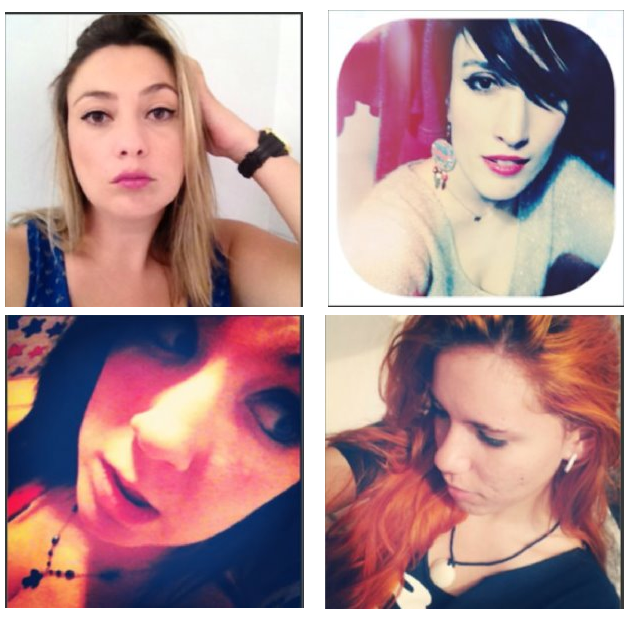
\includegraphics[width=25em]{res_vgg.png}}
			\caption{Results of image enhancement (vgg)}
			\label{res-fig}
		\end{figure}
		\begin{figure}[htbp]
			\centerline{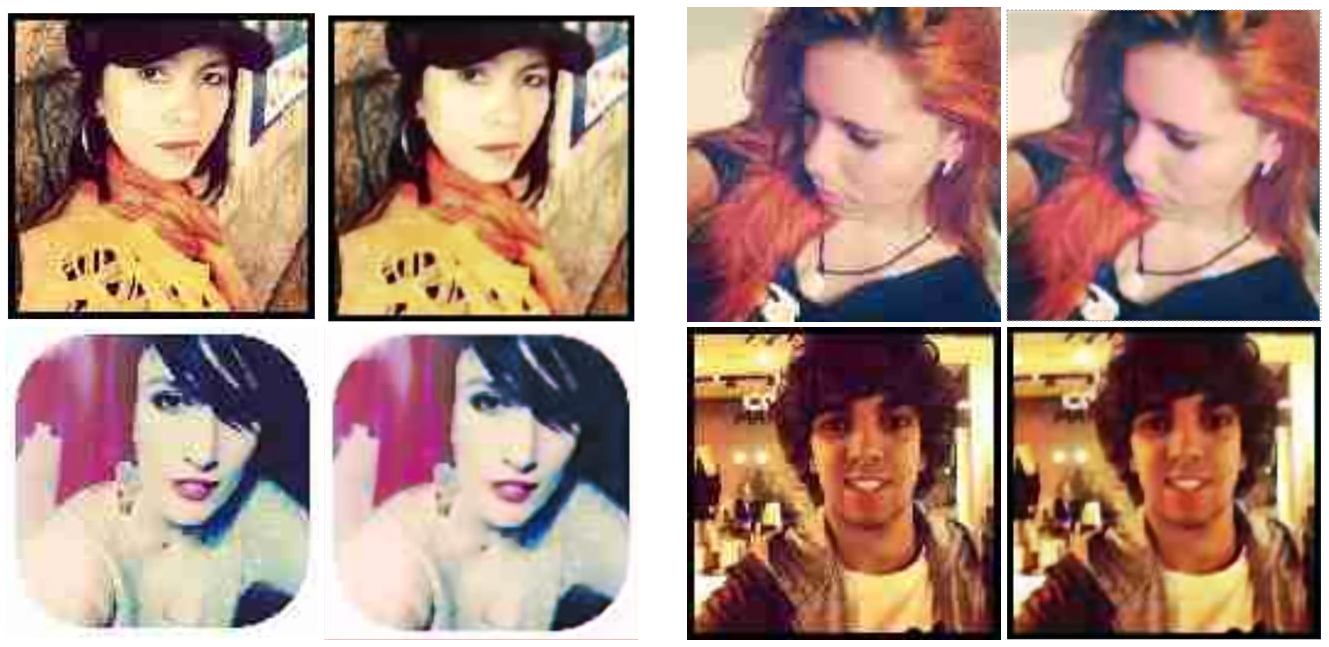
\includegraphics[height=12em, width=20em]{res_2.png}}
			\caption{Results of image enhancement (web-app) (zoom in to view difference)}
			\label{res2-fig}
		\end{figure}
	
	\section{Conclusion}
		Artificial Intelligence (AI) and Machine Learning(ML) have made a lot of progress and in many areas AI and ML models have even managed to outperform humans. With active research in this field, the performance of models is bound to improve further.
		\par The independent study undertaken manages to use such developments in ML to apply it the problem of enhancing low resolution images. The model was trained on dataset containing images of people and was able to perform reasonably well in the low resolution images it was tested with. With improvements to the model, it can also find commercial application which can be run in smartphones. A lot of users have their images stored in the cloud. The service providers tend to use compression to save space, sacrificing some quality in this process, so when the user downloads her/his images locally, super-resolution algorithms can be run to convert them back to high quality images.
		\par The study concluded with the creation of ML models that can be imported by other applications to directly perform image enhancement or can be used by other models through transfer learning. A basic web application was also created that can be used to perform image enhancements by a user.
		
	\section{Drawbacks}
		Some of the drawbacks of the current implementation include:
		\begin{itemize}
			\item The algorithm current can output to a maximum resolution of $512 * 512$ pixels. It is due to lack of computational resources during training.
			\item The algorithm only works for low resolution images (preferably below $384 * 384$ pixels). Giving an image of larger resolution $>(512 * 512)$ will result in the output image having lower quality.
			\item The web application is not able to use the up-sampler based on VGG architecture. Hence it is not as accurate and can lead to over-softening of images which look less sharp.
			\item Since the model was trained on a relatively small dataset (due to hardware resources), it may not output good quality output for images of certain scenes (e.g. overexposed scenes). 
		\end{itemize}
	
	\section{Future Score}
		The current implementation may be improved in the following way:
		\begin{itemize}
			\item The output resolution of images may be increased on more powerful hardware.
			\item The training loop can be extended to more cycles that may result in better output images.
			\item The size of the training dataset can be increased for better learning by the model.
			\item The underlying architectures (e.g. VGG16, ResNet34) can be replaced with more extensive architectures (e.g. VGG19, ResNet101, DenseNet161, etc.). This may result in better output with sharper images. However these architectures would require more powerful hardware to train.
			\item The web application that was created has been deployed locally. For better reachability, it can be hosted in Cloud Services like Amazon Web Services (AWS) and made public for anyone to use on the internet.
		\end{itemize} 
		\par Apart from modifications to the existing model, other models can also be explored that may or may not use GANs. Some models that provide better results include:
		\begin{itemize}
			\item Using Perceptual Loss Functions as described in the paper by Christian Ledig et al.\cite{b19}.
			\item Use Automated Texture Analysis as described by the paper by Mehdi S. M. Sajjadi et al.\cite{b20}.
			\item fastai super resolution implementation using VGG16 and having multiple training loops, each time with images of higher resolution, i.e. first training with images of size $(64 * 64)$, followed by images of size $(128 * 128)$, followed by images of size $(256 * 256)$, and so on. An implementation of the same can be found \href{https://nbviewer.jupyter.org/github/fastai/course-v3/blob/master/nbs/dl1/lesson7-superres.ipynb}{here}.
		\end{itemize}
		
	\section*{Acknowledgment}
		I express my gratitude to Dr. Pawan Kumar for providing with the opportunity to take PG-Independent Study under his guidance. During the course of the study, Dr. Pawan provided ample freedom to explore the field of study apply my own approach. Dr. Pawan also provided necessary guidance when required. The independent study helped me learn more about Generative Adversarial Networks, how they can be implemented and how to use ML models with more traditional programs like web applications.
		
	
	
	\begin{thebibliography}{30}
		\bibitem{b1} {Goodfellow}, Ian J. and {Pouget-Abadie}, Jean and {Mirza}, Mehdi and {Xu}, Bing and {Warde-Farley}, David and {Ozair}, Sherjil and {Courville}, Aaron and {Bengio}, Yoshua, ``Generative Adversarial Nets'', arXiv e-prints, \url{https://arxiv.org/pdf/1406.2661.pdf}
		\bibitem{b2} ``Generative Adversarial Network'', Wikipedia, the free encyclopedia, \url{https://en.wikipedia.org/wiki/Generative\_adversarial\_network}
		\bibitem{b3} Alec Radford, Luke Metz, Soumith Chintala, ``Unsupervised Representation Learning with Deep Convolutional Generative Adversarial Networks'', arXiv e-prints, \url{https://arxiv.org/pdf/1511.06434.pdf}
		\bibitem{b4} Martin Arjovsky, Soumith Chintala, Léon Bottou, ``Wasserstein GAN'', arXiv e-prints, \url{https://arxiv.org/pdf/1701.07875.pdf}
		\bibitem{b5} Min Lin, ``Softmax GAN'', arXiv e-prints, \url{https://arxiv.org/pdf/1704.06191.pdf}
		\bibitem{b6}  Kevin Su, ``Introduction to Image Super-resolution'', \url{http://www.cs.utsa.edu/~qitian/seminar/Fall04/superresolution/SR_slides_xsu.pdf} 
		\bibitem{b7} Jeremy Howard et al, ``fastai'', \url{https://docs.fast.ai/}, \url{https://www.fast.ai/}
		\bibitem{b8} NVlabs, ``Flickr-Faces-HQ Dataset (FFHQ)'', \url{https://github.com/NVlabs/ffhq-dataset}
		\bibitem{b9} Center for Research in Computer Vision, ``Selfie Data Set'', University of Central Florida \url{https://www.crcv.ucf.edu/data/Selfie/}
		\bibitem{b10} Olaf Ronneberger, Philipp Fischer, Thomas Brox, ``U-Net: Convolutional Networks for Biomedical Image Segmentation'', arXiv e-prints, \url{https://arxiv.org/pdf/1505.04597.pdf}
		\bibitem{b11} Kaiming He, Xiangyu Zhang, Shaoqing Ren, Jian Sun, ``Deep Residual Learning for Image Recognition'', arXiv e-prints,  \url{https://arxiv.org/pdf/1512.03385.pdf}
		\bibitem{b12} ``Mean squared error'', Wikipedia, the free encyclopedia, \url{https://en.wikipedia.org/wiki/Mean_squared_error}
		\bibitem{b13} ``Cross entropy'', Wikipedia, the free encyclopedia, \url{https://en.wikipedia.org/wiki/Cross_entropy}
		\bibitem{b14} Neurohive, ``VGG16 – Convolutional Network for Classification and Detection'', \url{https://neurohive.io/en/popular-networks/vgg16/}
		\bibitem{b15} ``Structural similarity'', Wikipedia, the free encyclopedia, \url{https://en.wikipedia.org/wiki/Structural_similarity#Multi-Scale_SSIM}
		\bibitem{b16} ``Peak signal-to-noise ratio'', Wikipedia, the free encyclopedia, \url{https://en.wikipedia.org/wiki/Peak_signal-to-noise_ratio}
		\bibitem{b17} ``Least absolute deviations'', Wikipedia, the free encyclopedia, \url{https://en.wikipedia.org/wiki/Least_absolute_deviations}
		\bibitem{b18} ``L1 norm'', Wikipedia, the free encyclopedia, \url{https://en.wikipedia.org/w/index.php?title=L1_norm&redirect=no}
		\bibitem{b19} Christian Ledig, Lucas Theis, Ferenc Huszar, Jose Caballero, Andrew Cunningham, Alejandro Acosta, Andrew Aitken, Alykhan Tejani, Johannes Totz, Zehan Wang, Wenzhe Shi, ``Photo-Realistic Single Image Super-Resolution Using a Generative Adversarial Network'', arXiv e-prints, \url{https://arxiv.org/pdf/1609.04802.pdf}
		\bibitem{b20} Mehdi S. M. Sajjadi, Bernhard Schölkopf, Michael Hirsch, ``EnhanceNet: Single Image Super-Resolution Through Automated Texture Synthesis'', arXiv e-prints, \url{https://arxiv.org/pdf/1612.07919.pdf}
	\end{thebibliography}
	
	
\end{document}